\documentclass[12pt]{article}
\usepackage[utf8x]{inputenc}
\usepackage[colorinlistoftodos]{todonotes}
\usepackage[bookmarks=true]{hyperref}
\usepackage{float}
\usepackage{placeins}
\usepackage{listings}
\usepackage{enumitem}
\usepackage{marvosym}
\usepackage{lmodern,textcomp}
\usepackage{amsmath}
\usepackage{algorithm}
\usepackage{algorithmic}

\hypersetup{pdftitle={Princing And Advertising},
	pdfauthor={Andrea Furlan, Cosimo Russo, Giorgio Ughini},        
	pdfsubject={DIA},
	colorlinks=true,
	linkcolor=blue,
	citecolor=blue,
	filecolor=black
	urlcolor=purple,
}

\begin{document}
	\begin{titlepage}
		\newcommand{\HRule}{\rule{\linewidth}{0.7mm}}
		\center
		
\includegraphics{PolimiLogo.png}\\[1cm]
		
		\textsc{\LARGE Project Report Document}\\[1cm]
		\textsc{\large Data Intelligence Application - A.Y. 2019-2020}\\[1cm]
		\HRule \\[0.4cm]
		{ \huge \bfseries Pricing and Advertising}\\[0.15cm]
		\HRule \\[1.5cm]
		{\large Authors  \hfill ID Numbers}\\[0.4cm]
		{\large Andrea \textsc{Furlan}  \hfill 944774}\\[0.2cm]
		{\large Cosimo \textsc{Russo}  \hfill 945891}\\[0.2cm]
		{\large Giorgio \textsc{Ughini} \hfill 944710}\\[2cm]
		{\large \today  \hfill Version 1.0}
		\vfill
	\end{titlepage}
	\clearpage
	{\hypersetup{hidelinks}\tableofcontents}
	\clearpage
	\section{Introduction}
	\subsection{The Product}
	\begin{figure}[!htp] 
	\begin{flushleft}
		In this project we would like to focus our attention on a specific product: a luxury scarf. We decided to take into consideration this item because it's a seasonal product that is more searched by its buyers in the cold seasons and less demanded during the summer days. This periodic variation of the users' interests is an interesting input to take in consideration during our analysis. We decided to use as a subject the classical Louis Vuitton brand logo scarf, well known and trending in our country.
	\end{flushleft}
	\centering
	
\includegraphics[width=0.8\linewidth]{sections/productLogo}
	\caption{Louis Vuitton Brand Logo Scarf.}
\end{figure}
\clearpage
	\subsection{The Classes of Users}
	Given that the product we want to study generates more interest in women rether than in men, we decided to focus our studies on women only. We also came to the conclusion that since a luxury scarf is usually bought from the middle and the upper class person, a minimum family yearly income bound was necessary to set our focus on only the users that are able to generate more impact on the analysis. We set this bound at 80.000 \EUR{} gross. Finally we thought that since trends can vary among countries, considering only the Italian population was the most reasonable choice to avoid unwanted biases.
The binary features that we decided to observe on our users are:
\begin{itemize}
	\item \textbf{With/Without children}:\@ To better observe the impact that a son can have in buying a luxury item
	\item \textbf{Living in the North/South of Italy}:\@ To better observe the impact that the climate and the local traditions can have in buying an item that is useful only in certain seasons.
\end{itemize}
The distribution of our customer base is described in the following pie chart:
\makebox[\textwidth][c]{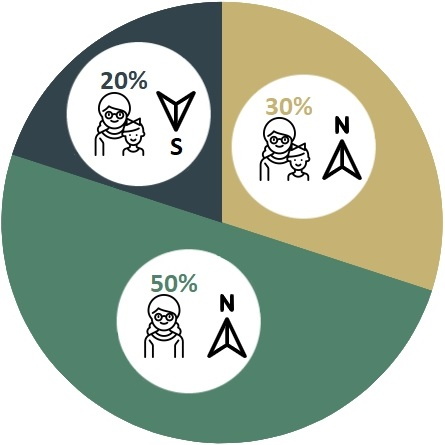
\includegraphics[width=0.7\textwidth]{sections/images/usersImage3}}
%\makebox[\textwidth][c]{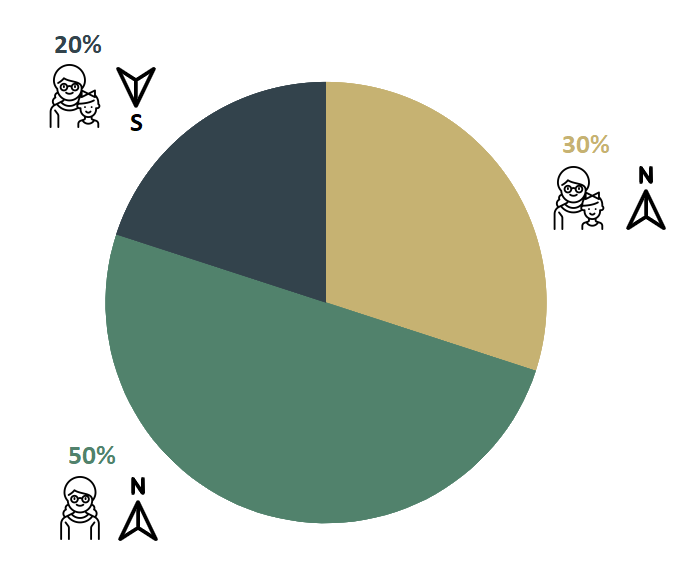
\includegraphics[width=0.9\textwidth]{sections/images/usersImage}}
	\subsection{The Conversion Rate Curves}
	Since the Louis Vuitton brand logo scarf is classified as a luxury good, we hypothesised the three conversion rate curves to have non-negative-slope and reaching their peak near the \EUR{200-250} range. \\These curves are the curves that rule the environment of our experiment.\\An illustration of our hypothesised conversion rate curve is presented below:\newline
\makebox[\textwidth][c]{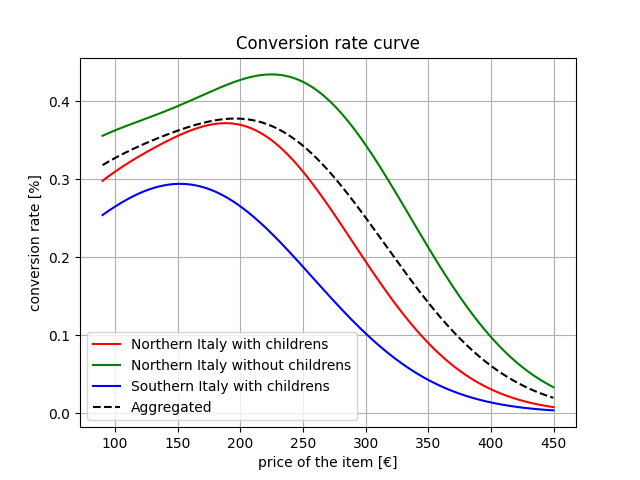
\includegraphics[width=1.1\textwidth]{../curves/real_curves/conversion_rate_curve}} 
\clearpage
	\subsection{The Subcampaigns}
	In order to advertise our product we outlined three different sub-campaign each with a unique aspect and a particular type of user as a target. The three sub-campaigns are focused on:
\begin{itemize}
	\item \textbf{The Quality Of The Product}:\@ \newline Targeting the women with children living in the north of Italy.
	\item \textbf{The Social Impact Generated By The Product}:\@ \newline Targeting the women without children living in the north of Italy.
	\item \textbf{The Peculiarity And The Uniqueness Of The Product}:\@ \newline Targeting the women with children living in the south of Italy.
\end{itemize} 
An idea of how the ads could be is the following: \newline\\\\
\makebox[\textwidth][c]{
\includegraphics[width=1.2\textwidth]{sections/images/ad1}}
\makebox[\textwidth][c]{
\includegraphics[width=1.2\textwidth]{sections/images/ad2}}
\makebox[\textwidth][c]{
\includegraphics[width=1.2\textwidth]{sections/images/ad3}}

	\subsection{The Abrupt Phases}
	As we said in the first section, the product taken into analysis is a seasonal item. Using Google Trends, we were able to identify the region of maximum and minimum interest of the users regarding a Louis Vuitton scarf. In the graph below is clear that this product is searched primarily in the cold seasons and it is year after year more demanded by the customers. In the chart the x-axis represents a five year time period while the y-axis represents the popularity of the keywords "Louis Vuitton Scarf" searched on Google (100 is the moment of maximum interest while 0 is the minimum).
\makebox[\textwidth][c]{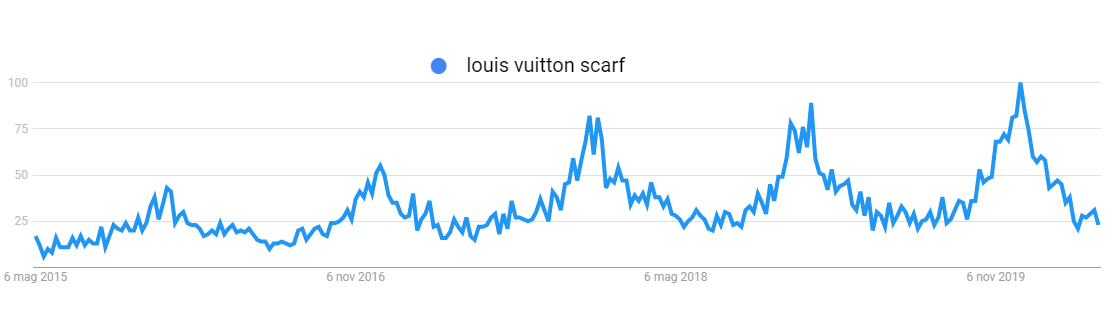
\includegraphics[width=1.2\textwidth]{sections/images/trend}}
Based on the diagram we decided to divide the year in four periods of time, each one underlining a different phase.\newline\\
\makebox[\textwidth][c]{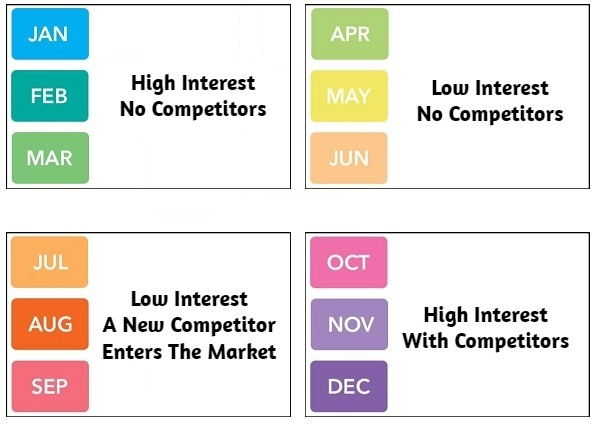
\includegraphics[width=0.8\textwidth]{sections/images/months}}
In order to better understand our reasoning behind the decisions that brought us to choose as graphs for the four different phases the ones showed below, is important to notice some remarks. \\In the first phase (Jan-Feb-Mar) the growth of the curve is almost linear, since there are no competitors that can interfere with our advertising of the product, but still there is a large pool of users to influence, since it is a phase of high interest of the product.\\ In the second phase (Apr-May-Jun) instead, since in these months the interest about the item is low, there will be less people interest in the scarf, therefore the impact that a higher budget allocated to the ads can make is less relevant that the impact that it can produce on a high interest phase. Based on this assumption we decided that the graph for the second phase should have a more remarkable growth with a small budget allocated to the ads, settling to much more slower growth as the budget significantly increases. \\In the next phase (Jul-Aug-Sep), when the new competitor enters the market, the graph should be different in the low budget allocated range respect to the second graph, while maintaining a similar profile in the high budget allocated range. The cause is the following: since we need to beat the competition in order to sell our product, we will struggle to do so allocating a small amount of money to the advertisement, while instead allocating a sufficient amount of money, we should be able to attract user to us as if there was not a competitor in the market. \\Finally, in the last phase (Oct-Nov-Dec) we focussed on the fact that since it is an high interest phase, but this time with a competitor that challenges us, the budget that needs to be allocated to the sub-campaigns still needs to be a considerable amount if we want to attract a sufficient number of users as in the third phase, but in this period the pool of users that can be reached is much wider, translating in a more linear curve in the high budget allocated range with respect to the third phase.\\
Taken into consideration our reasoning, the images below will present the structure of the probability distribution over the daily number of clicks for every value of budget allocated to that sub-campaign.\\
\makebox[\textwidth][c]{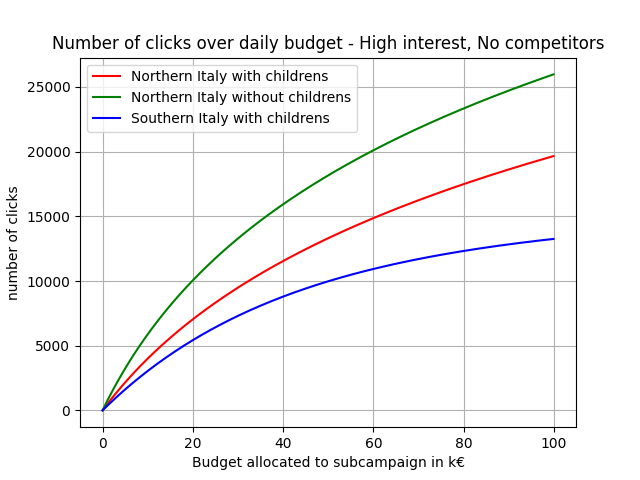
\includegraphics[width=0.85\textwidth]{../curves/real_curves/daily_clicks_10}} 
\makebox[\textwidth][c]{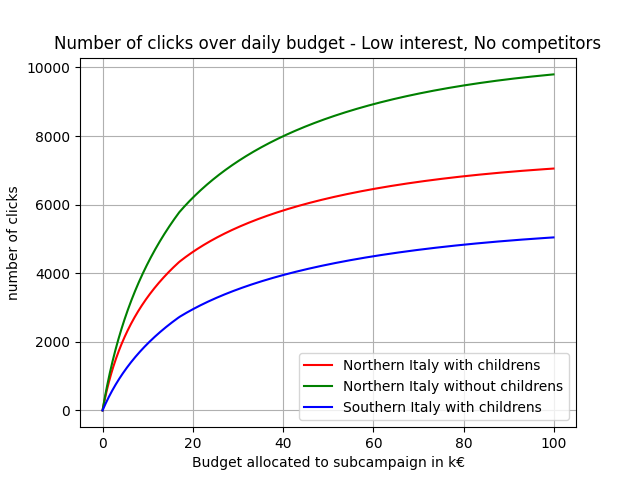
\includegraphics[width=0.85\textwidth]{../curves/real_curves/daily_clicks_00}} 
\makebox[\textwidth][c]{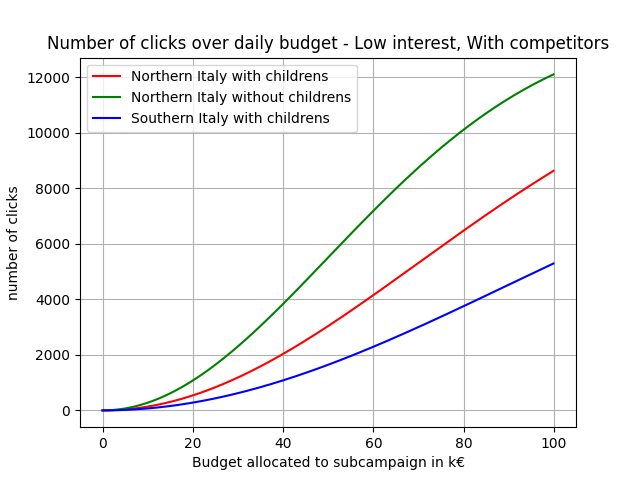
\includegraphics[width=0.85\textwidth]{../curves/real_curves/daily_clicks_01}} 
\newline\\\\
\makebox[\textwidth][c]{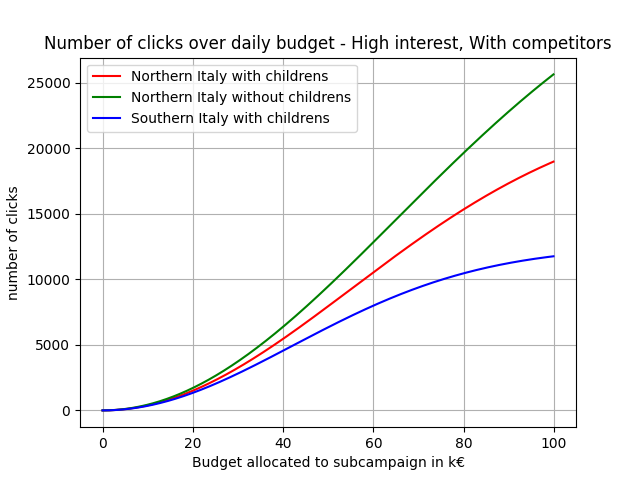
\includegraphics[width=0.85\textwidth]{../curves/real_curves/daily_clicks_11}} 
	\subsection{The code}
	In this document we will refer to algorithms implemented in Python which code can be found at LINK-AL-CODICE.	
	\newpage
	\section{Case study and Algorithms}
	
	\subsection{Budget allocation with only one phase}
	The first step of our project was focused on the budget allocation over the three subcampaigns and had as goal the maximization of the total number of clicks.
In this first stage, for simplicity, only one phase is considered.
	\subsubsection{Experiment setting}
	The first step of the process is the definition of the size of the experiments, in particular:
\begin{itemize}
	\item \textbf{The number of arms}:\@  the higher it is, the more likely is the chance of exploring
	arms that are close to the optimal arm. On the other hand, having more arms
	implies that the optimization horizon will be required to be longer to allow a
	proper exploration of all the arms.
	\item \textbf{The optimization horizon}:\@  this is the amount of time that will be spent
	running the price optimization algorithms. The longer this is, the more are
	the possibilities that can be explored. However, exploring more possibilities
	causes to have a bigger loss - or regret - in the initial phases of the exploration.
\end{itemize} 
It appears clear that the the two quantities depend one on each other
and represent the key of the optimization. A reasonable optimization horizon is
one year. Indeed, the interest that people have for our product behaves in the same way every
year, the phases alternate cyclically and the period of the cycle is one year.
Thus, as long as we are able to collect enough data during one year, it makes no
sense to extend the optimization horizon to a time that is longer than this.
The choice of the number of arms is an hyper-parameter that the corporate should input, by setting the minimum budget to allocate to each subcampaign ($min-budget$), the maximum one ($max-budgets$) and the granularity ($step$).
\\For this experiment, we set the same minimum budget for all subcampaign (equal to \texteuro1000) but different upper bound as we consider the company to have (very low) prior information about their classes on user. The upper bound for the budget was then set to \texteuro5400, \texteuro5800 and \texteuro5200 for the three categories of users, reflecting the fact that the company can afford to spend more for his top spending users.
As a luxury brand, the company decided to have a high granularity in the budget allocation, to exploit at best all the advantages of the CMAB approach in finding the best allocation.
\\Indeed, the company could even have some prior information about users behaviour, but for sure it cannot know what is the best choice for the budget allocations as it depends upon too many factors.
\\In particular, $step=2$ that means the allocation of budget has a granularity of \EUR{200}. With the same granularity but different allocation range, each GP Learner resulted in a different number of arms (respectively 22 arms for North/WithChildren, 24 arms for North/WithoutChildren and 21 arms for South/WithChildren).
	\subsubsection{Gaussian Process Combinatorial Multi-armed Bandit}
	The pseudo code of the algoritm we implemented is as follow.
\begin{algorithm}
	\caption{Gaussian Process CMAB}
	\begin{algorithmic}[1]
		\STATE $J\gets ${ all classes of users}
		\FOR{$j \in \{1,...,J\}$}
		\STATE Sample j-th GP-Learner
		\STATE Add row to knapsack matrix
		\ENDFOR
		\STATE Optimize knapsack matrix
		\STATE Play selected superarm
		\STATE Update GP-Learners model
	\end{algorithmic}
\end{algorithm}
	\newpage
	\subsubsection{Results}
	The experiment shows that after only 7 days of exploration, the corporate could start to exploit the best arms, converging to the optimal one after about half a month.
\newpage
The regret chart that resulted from this experiment is as follows:\\
\makebox[\textwidth][c]{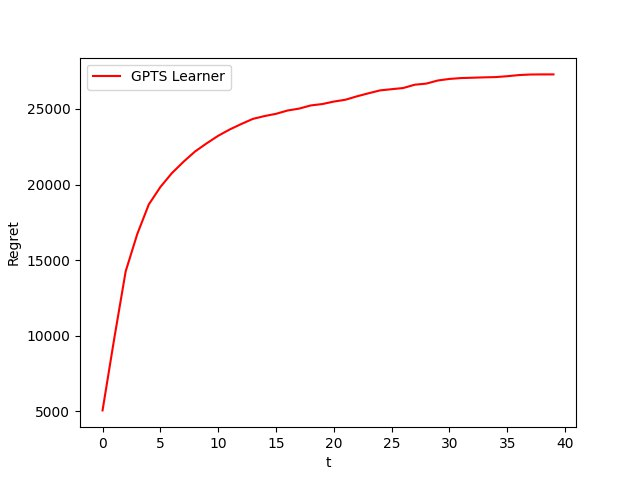
\includegraphics[width=1\textwidth]{../curves/results/budgetallocation_stationary_results}}
	\newpage
	\subsection{Budget allocation with four phases}
	After having analized the budget allocation over the three subcampaigns considering only one phase, we are moving to a more general context.
\\In particular, we supposed the existance of four different phases in a year, that are:
\begin{itemize}
	\item \textbf{JAN-FEB-MAR}: These months can still be considered "cold months", so the \emph{interest} in a scarf \emph{is still high}. In addition, we suppose that \emph{no competitor} will launch a new product in these months because that competitor would miss the OCT-NOV-DEC high interest phase.
	\item \textbf{APR-MAY-JUN}: In these spring months \emph{the interest} in a scarf \emph{becomes low} as temperature arises. Of course, \emph{no competitor} are present for the same motivation as above.
	\item \textbf{JUL-AUG-SEP}: If a \emph{new competitors wants to join the market}, the best time of the year to do so is the late-summer/beginning of fall. In this way, even if this phase can still be considered a \emph{low interest phase}, the competitor could start to promote its product to be ready for late-fall and winter.
	\item \textbf{OCT-NOV-DEC}: A \emph{new competitor has joined the market} in the previous months and now the customer base has to take a decision on which is their favourite, possibly based on the marketing strategy each party encompass. These cold month will be, naturally, a \emph{high interest phase}.
\end{itemize}
	\subsubsection{Experiment setting}
	In case of non-stationary environment, it is important to define a
proper value for the sliding window, that is, the length of the buffer where the latest
collected samples are stored. We considered two different formulas to compute a
reasonable sliding window length, which pros and cons are reported below:

\begin{itemize}
	\item \textbf{Unknown environment}:\@  This is the basic formula for the computation of the window length. It only considers the number of interactions T our algorithm is going to perform
	with the environment.
	$$SW_1 = \sqrt{T}$$
	It is a very simple formula, altough with large numbers of arms it leads to bad performances, as it does not take it into account.
	
	\item \textbf{Some environment knowelge}:\@  Provided that all the phases of the demand curve have the same length so that they are uniformly distributed over the time horizon, we’re setting the sliding window size equal to a third of this length, in 	order to keep re-exploring the "old" arms at least 2 time inside the same phase but to be more ready in case of a abrupt change (like in correspondence of the beginning
	of a new phase).
	$$SW_2 = \dfrac{T}{3F}$$
	This is a very simple formula, tailored for a specific case, the phases should be uniformly distributed over the time horizon
	and their lengths have to be equal, which is not always the case.	
\end{itemize} 

We supposed that the compay could have a small prior information about the distribution of the phase that could come from previous campaign analisys or other sources.
\\As the phases are uniformly distributed and we know the number of it and the optimization horizon, we implemented the second formula for the Sliding Window lenght that resulted in:
$$SW = \dfrac{365}{4*3} = 1 month$$
This is a reasonable amount of time as, provided the existance of 4 phases in a year, each phase would last 3 month and using this $SW$ time we're sure that after a month a new phase has begun, no more dirty data are considered.
	\subsubsection{Sliding-Window Gaussian Process Combinatorial Multi-armed Bandit}
	The pseudo code of the algoritm we implemented is as follow.
\begin{algorithm}
	\caption{Gaussian Process CMAB}
	\begin{algorithmic}[1]
		\renewcommand{\algorithmicrequire}{\textbf{Input:}}
		\REQUIRE $\tau$ sliding window size, $J$ classes of users
		\FOR{$day \in \{1,...,T\}$}
			\FOR{$j \in \{1,...,J\}$}
			\STATE Sample j-th GP-Learner($\tau$)
			\STATE Add row to knapsack matrix
			\ENDFOR
			\STATE Optimize knapsack matrix
			\STATE Play selected superarm
			\STATE Update GP-Learners model($\tau$)
		\ENDFOR
	\end{algorithmic}
\end{algorithm}
\\The update of the GP-Learner's model performed at time $\tau$ is achieved by adding the collected reward to the reward space and then discarding the least element if the current time exceeds $\tau$.
	\subsubsection{Results}
	We compare the behaviour of applying the same GPTS Learner of the previous experiment (this time in presence of all the phases) with the performance of the SW GPTS Learner.
\\The experiment shows that the standard GPTS performs better in the first and the second phase of the year.  The better performance in the first phase is due to the fact that while the SW-GPTS always keep at maximum 1 month of memory, the basic GPTS keeps collecting samples. 
\\While comparing the second phase we can see that the performance of convergence of the two learners is quite the same. The standard GPTS does not suffer too much the fact that the first phase has ended because it is only a transition bethween a high interest phase and a low interest phase and therefore the budget allocation does not change too much among the classes of users.
\\The presence of a competitor change a lot into the budget allocation. It is not enougth to allocate the budget with respect of the average client of the brand because our company now needs to invest more on a class to gain the same results on it, but the budget is limited. A choice is then needed in the third and the fourth phases and this explains the different behaviour. 
\\After about one month of exploration the SW-GPTS is able to converge in this new phase while we see that the basic GPTS will not converge anymore from now on: the sample collected in the preceding months weights too much on the choice of the budget allocation.
\\The regret chart that resulted from this experiment and the reward collected for each day are reported in the below figures.\\
\makebox[\textwidth][c]{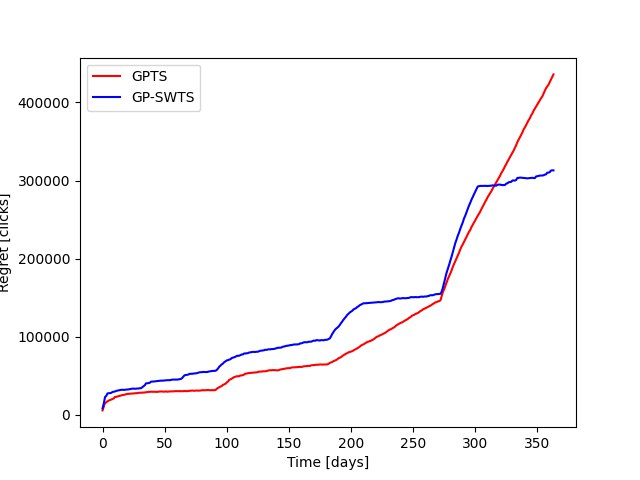
\includegraphics[width=0.85\textwidth]{../curves/results/swgpts-tmp-regret}}
\newpage
\makebox[\textwidth][c]{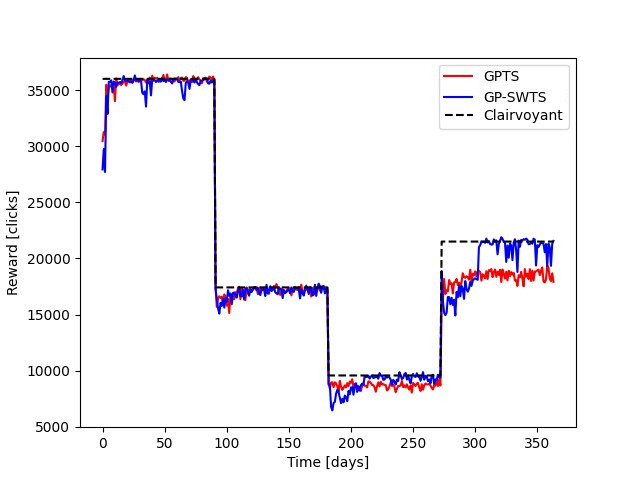
\includegraphics[width=0.85\textwidth]{../curves/results/swgpts-tmp-reward}}
	\newpage
	\subsection{Learning Algorithm for Pricing}
	In this section, we describe the learning algorithm that we used to maximize the number of purchases made by users that have reached our website by clicking on ads.

\subsubsection{Assumptions}
\begin{enumerate}
    \item There is only one phase
    \item The allocation of the budget over the three subcampaigns is fixed
\end{enumerate}

\subsubsection{Setup of the experiment}
3 Thompson Sampling learners are used, one for each class of users. Since the users arrive on the purchase page by clicking on the ads, we assume that we can differentiate them by their class, thus proposing a different price to each user.

To satisfy assumption (1), the algorithm runs for a limited number of days, 45, enough to provide a significant result.

The average number of users that arrive per day are taken from the results of the previous point, which optimizes the budget in the fourth phase and maximizes the number of clicks. It returns the following average number of daily clicks: $C=[1800, 12000, 350]$. For this experiment, we will use these values as the daily average number of clicks, with a variance that is proportional to each value: $Var_i = C_i / 4$ $\forall{i} \in \{1,2,3\}$.

Since the optimization of the budget is made once a day and depends on the price chosen, also the price (for each class of users) is chosen once per day.

The minimum and maximum prices (0, 400) are the same for all the classes of users. The same goes for the number of arms, for which we tested various configurations ranging from 4 to 10 arms to see which one provided the best result.

\subsubsection{The algorithm}
The high-level pseudo code of the algorithm is shown in Algorithm \ref{alg:ts_pricing}.

Each TS learner is responsible for a class of users. Each day, the 3 learners pull the best price from their beta distributions. The prices are then proposed to all the users that arrive to the website on that day after clicking on the ads. At the end of the day, the learners are updated with the number of successes (purchases) for each class.

\begin{algorithm}
    \caption{TS learners for pricing}
    \label{alg:ts_pricing}
	\begin{algorithmic}[1]
        \STATE $J\gets ${ all classes of users}
        \STATE $T\gets ${ 45 days }
        \STATE $regret\gets ${0}
        \FOR{$day \in T $}
		\FOR{$j \in \{1,...,J\}$}
		\STATE $price\gets ${Draw a price from the j-th TS learner}
        \STATE $successes\gets ${number of buys with pulled price}
        \STATE $failures\gets ${clicks[j][day] - successes}
        \STATE $reward\gets ${successes * price}
        \STATE regret += optimum - reward
        \STATE TS[j].update(pulledArm, successes, failures)
        \ENDFOR
        \ENDFOR
	\end{algorithmic}
\end{algorithm}

Some remarks:
\begin{itemize}
    \item on line 6, to draw a price means that for each arm $a$ we pull a sample $\theta_a$ from the beta distribution, and then return the price $p_a$ of the arm that offers the best reward, that is $p_a = \underset{p_a}{argmax} \{p_a * \theta_a\}$
    \item on line 11 the update of the TS learner consists in updating the beta parameters of the arm pulled, in the following way: $(\alpha, \beta) += (successes, failures)$
\end{itemize}

\subsubsection{Choice of the best arm}
The following results come from averaging over 1000 experiments.

We tested the experiment with several numbers of arms. For each number $n$ of arms, draw the $n$ prices equally spaced in the interval and run the experiment, calculate the regret and the reward and use them to choose the best number of arms.

The first image shows the cumulative regret using different arms, ranging from 3 to 7.
Given the limited time-span, the best result is provided by a low number of arms, which converges more rapidly to the best arm.

However, since in the calculus of the regret we use as clairvoyant the best possible arm, we know how fast the learner converges but not how much money we would be losing in the ideal case in which we could use an infinite number of arms. For this reason, we set up another experiment in which we calculate the reward and compare it with the clairvoyant reward that, in this case, corresponds with the reward that we would get if we chose, for each class, its actual best price.

\begin{figure}[]
    \centering
    
    \caption{Reward of the TS Learner}
    \label{Reward of the TS Learner}
\end{figure}

As the image shows, using 3 arms does not offer a good reward. The best number of arms that comes out from our experiment is 4, which is aligned with the theoretical expection that we have with a period of 45 days.

\subsubsection{Results}
With 4 arms, we have a reasonably fast convergence to the best arm and enough arms to pull a price that is close enough to the clairvoyant to obtain a good reward.
	\newpage
	\subsection{Context Generator Algorithm}
	The next few slides focus on a context generation algorithm for the pricing when the budget allocated to each single sub-campaign is fixed. This means that we focus on trying to understand the different behaviours that the three class of users studied may follow. Since the three types of users are different by means of purchasing power, price discrimination may be important to further increase the reward instead of considering the users as a single class. Therefore, our goal is to understand whether or not it can be useful to divide the users in the various classes. From the theory we know that it is worth splitting if the lower bound on the probability that context 1 occurs plus the probability that context 2 occurs should be greater or equal to the lower bound on the best expected reward for the context not yet splitted; we test this condition and eventually perform the split every 7 days, that is a week.
\subsubsection{Setup of the experiment}
The algorithm requires to define some inputs from which the context generation will begin. In particular is important to define:
\begin{itemize}
	\item \textbf{The bandit algorithm to implement:} Empirically the best algorithm to adopt is almost all the scenarios the Thompson Sampling algorithm, so we opted to it in order to perform our experiment.
	\item \textbf{The number of arms:} As stated in the chapter before, the number of arms that have a reasonably fast convergence to the best arm and enough arms to pull a price that is close enough to the clairvoyant are 4,5,6 or 7. In this scenario, the algorithm uses 6 arms.
	\item \textbf{The number of clicks per day:} The more clicks per day on the ads, the more the algorithm will be able to exploit the disaggregation faster since there will be a huge number of data to work with. We tried to choose a number as close as possible to what it could be a real number of users that click daily on ads like ours. We opted to 17000 clicks per day, based on the  optimization algorithm presented in the chapter before.
	\item \textbf{The time span of the experiment:} It is considered a time span of 90 days that is because we are considering the experiment to the take place on the first phase (Jan-Feb-Mar).
\end{itemize}
Since the process involves some randomness, the splits can be done in different order and in different weeks, and the graphs shown as an output may differ. It is important to notice that since there are only 6 arms to explore, the splits always happen in the first weeks, while in a setting with more arms the splits can happen later in time.
\subsubsection{The Algorithm}
A pseudo code that describes how the algorithm works is this:\\

\begin{algorithm}
	\caption{Context Generator Algorithm}
	\begin{algorithmic}[1]
		\renewcommand{\algorithmicrequire}{\textbf{Input:}}
		\REQUIRE $T$ : time span of the experiment, $C$ : number of clicks per day
		\FOR{$1 \leq t \leq T$}
		\FOR{$1 \leq c \leq C$}
		\FOR{$context \in Contexts$}
		\FOR{$usert ype \in context$}
		\STATE $sort \gets ${ Draw the choice of the user from the binomial}
		\STATE $successes \gets ${ Update the number of successes for that user and context}
		\STATE $failures \gets ${ Update the number of failures for that user and context}
		\ENDFOR
		\STATE $reward \gets ${ Update the reward value for the day}
		\ENDFOR
		\STATE $rewards \gets ${ Append the reward value for the day}
		\ENDFOR
		\IF{t mod 7 == 0} 
		\FOR{$context \in Contexts$}
		\FOR{$usert ype \in context$}
		\IF{split condition achieved}
		\STATE $c1, c2 \gets${ Perform the split}
		\ENDIF
		\ENDFOR
		\ENDFOR	
		\ENDIF
		\ENDFOR
	\end{algorithmic}
\end{algorithm}
\newpage
\subsubsection{Results}
After the 90 days period the graphs of the reward and the regret results as follow:\\\\\\\\\\\\\\\\
\makebox[\textwidth][c]{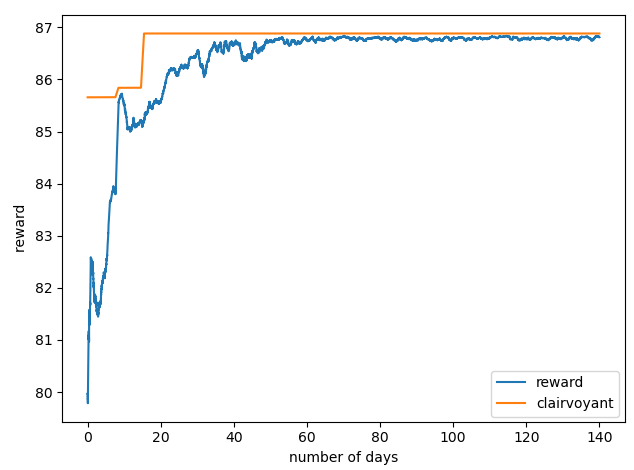
\includegraphics[width=0.9\textwidth]{../curves/results/context_generator_2000clicksperday_reward}}
\makebox[\textwidth][c]{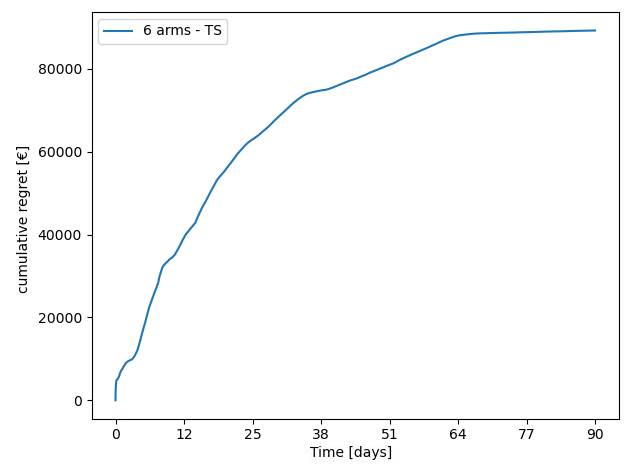
\includegraphics[width=0.9\textwidth]{../curves/results/context_generator_2000clicksperday_regret}}\\\\\\\\
By watching the clairvoyant plot, it is clear that the splits happened two times (expected since there are three class of users), the first one in the first week of the experiment, and the second one on the second week. \\The reward deviates more from the clairvoyant in the initial weeks, when the splits still need to happen and influence the computations of the following weeks, and later converges to the clairvoyant, once the shift to the splitted scenario occurs. \\Complementary, the cumulative regret graph shows an exponential and more substantial growth in the first weeks, and later settles after the splits have influenced the reward.
	\newpage
	\subsection{Optimization Algorithm}
	After studing the budget allocation and the pricing scenario separately, we imagined the union of the two, used in a real application of the selling of our scarf.
Indeed, we designed an optimization algorithm combining the allocation of budget and the pricing when \emph{the seller a priori knows that every subcampaign is associated with a different context} and charges a different price for every context.

The algorithm consists in a Combinatorial-MAB where the combinatorial part is very similar to the knapsack problem, where the value per click used in this problem depends on the pricing, that depends on the number of users of a specific class interested in buying the product.

The pricing and the advertising problem can, in this case, be decomposed since each subcampaign targets a single class of users. In this way, the computation of the value per click of a campaign depends only on the basis of the number of clicks generated by that specific subcampaign. 
	\subsubsection{Experiment setting}
	As this experiment is substantially the union of the budget and the pricing problem, and given that the problem can be decomposed, no new Learner is implmented here. Instead, a new Environment is created, as this time it should keep memory of the real behaviour of the users based on the budget allocated and of the real behaviour of the users based on the pricing chosen. The core of the experiment here is the set up of the two classes of Learners (GPTS Learner of the budgeting and the TS Learner for the pricing) in a way that they can work together.

Aside from the common variables \textit{TIME-SPAN}, \textit{N-CLASSES} and \textit{N-EXP}, in the main function we had to set up the parameter under the control of the company, that are:

\begin{itemize}
	\item \textbf{Budget bounds}: the variables min-budget and max-budget are arrays that contains the budget bount for the budget problem. In this case, the company has chosen to allocate a minimum budget of \EUR{1000} to each subcampaign while it can afford to spend more on its top class buyers, respectively \EUR{5400} for class 1, \EUR{5800} for class 2 and \EUR{5200} for class 3.
	\\\item \textbf{Pricing bounds}: with the algorithm we designed, it will be possible for the company to fix a different price for each category of users so it makes sense to give the possibility to the company to set different price bounds for each class of users. In this experiment, the company set the same bounds for all the classes \EUR{100}-\EUR{400} but the possibility to change is still possible by setting the parameters of the algorithm.
	\item \textbf{Maxmium budget}: this is the costraint needed for the knapsack-like problem that represent the maximum amount of money the company wants to spend. For this experiment this variable is set to \EUR{9000}.
	\item \textbf{Granularity}: as for the first experiment (the budgeting problem alone), the allocation of budget has a granularity of \EUR{200}. With the same granularity but different allocation range, each GP Learner resulted in a different number of arms (respectively 22 arms for North/WithChildren, 24 arms for North/WithoutChildren and 21 arms for South/WithChildren).
\end{itemize}
	\subsubsection{Gaussian Process Combinatorial Multi-armed Bandit}
	\begin{algorithm}
	\renewcommand{\algorithmiccomment}[2][.4\linewidth]{%
		\leavevmode\hfill\makebox[#1][l]{//~#2}}
	\caption{Optimization Algorithm}
	\begin{algorithmic}[1]
		\STATE $J\gets ${ all classes of users}
		\FOR{$day \in T$}
		\FOR{$j \in \{1,...,J\}$}
		\STATE $p \leftarrow \text{Sample(j-th TS)}$
		\COMMENT{Price}
		\STATE $a \leftarrow$ Get predicted conversion-rate given the pulled arm
		\STATE $c \leftarrow \text{Sample(j-th GPTS)}$
		\COMMENT{Number of clicks}
		\STATE $b \leftarrow \text{Budget(j-th GPTS)}$
		\COMMENT{Budget spent}
		\STATE $v \leftarrow \dfrac{p\cdot a\cdot c - b}{c}$
		\COMMENT{Value per click}
		\STATE Add row $v\cdot c$ to knapsack matrix
		\ENDFOR
		\STATE $a \leftarrow$ Optimize knapsack matrix
		\STATE $rew \leftarrow $ Play selected superarm $a$
		\STATE Update GPTS-Learners model
		\STATE Update TS-Learners model
		\ENDFOR
	\end{algorithmic}
\end{algorithm}
The pseudo code of the algoritm we implemented is as above, where the GPTS-Learners are those incharged of the budget problem and the TS-Learners are incharged of the pricing.

During the model update, an important consideration should also be taken into consideration: as problem can be decomposed, the optimal solution is the union of the three optimal rewards sub-solution (remember that the seller can set a different price for each class of user).

	\subsubsection{Results}
	The experiment shows that after only 10 days of exploration, the corporate could start to exploit good superarms, converging to the optimal one after about half a month.

This result is achieved because the combinatorial problem is solved in an exact way, thus increasing the execution time but lowering the additional regret. This is a reasonanble assumption as the corporate can run the algorithm over the night or in any time with low orders.
\\The approximation of the solution of the combinatorial problem would have saved just few minutes of computation but would have increased the regret of a non-trascurable amount of money, as a luxury brand cannot afford to sell products even with a sightly wrong price.
\\The cumulative regret when the algorithm learns both the conversion rate curves and the performance of the advertising subcampaigns is plotted as follows, along with its complementary reward chart that shows the reward at each time $t \in T$.
\\
\makebox[\textwidth][c]{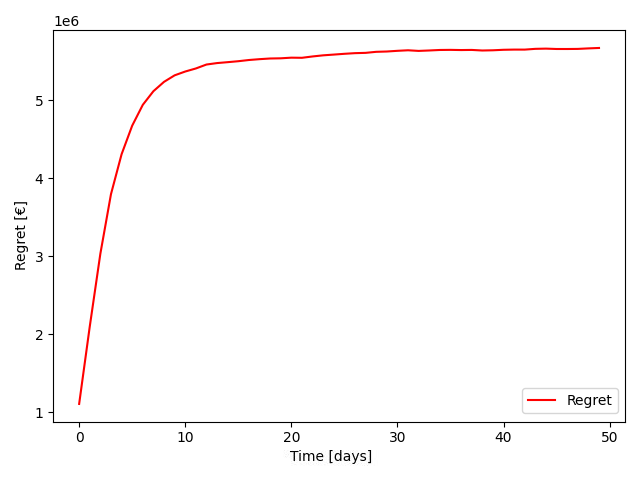
\includegraphics[width=0.9\textwidth]{../curves/results/bdgalloc_and_pricing_real_regret}}
\makebox[\textwidth][c]{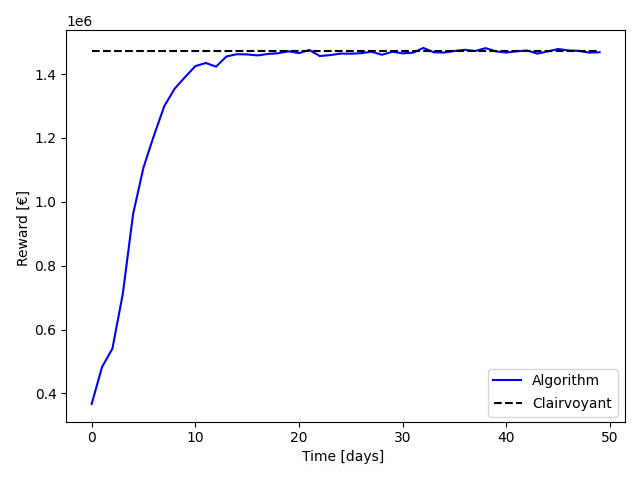
\includegraphics[width=0.9\textwidth]{../curves/results/bdgalloc_and_pricing_real_reward}}

	\newpage
	\subsection{Optimization Algortihm Constrained}
	In this final step, we will analyze the design of an optimization algorithm combining the allocation of budget and the pricing when the seller a priori knows that every subcampaign is associated with a different context and charges a unique price to all the classes of users.

\subsubsection{Assumptions}
\begin{enumerate}
    \item The optimal bid is automatically set
    \item Single phase
\end{enumerate}

\subsubsection{Setup of the experiment}
For this experiment we will consider a time span $T=50$ days. Other variables are:
\begin{itemize}
    \item Total budget $b_{tot}$ that can be used for advertising
    \item The array of possible budgets $B$, e.g. the arms of the GPTS learners. (We used the same array for all learners)
    \item The array of possible prices $P$, e.g. the arms of the TS learners. (We used the same array for all learners)
    \item $C=3$ classes of users
    \item Maximum budget for each subcampaign: $b_{max_i}, 1 \leq i \leq C$ (the minimum is 0 for all subcampaigns)
    \item Minimum and maximum prices, that we set equal to 100 and 400.
    \item $\theta$ an array of 3 elements that contains the price pulled by the 3 TS learners on each day
    \item $d_p$ the estimation of the demand curve at price p provided by the TS learner
    \item $clicks$ is a $C \times |B|$ matrix, in which the element $i,j$ corresponds to the estimated number of clicks for the i-th ad with budget $B_j$
    \item $vpc$ is a $C \times |B|$ matrix, in which the element $i,j$ is the estimation of the value of one click on an ad of class i if the budget is set to $B_j$.
    \item $b_{best}$ is an array of size $C$ in which the i-th element represent the best budget allocation for class i
    \item $r_{exp}$ is an array of size $C$, the i-th element contains the expected revenue of class i
    \item $r_{max}$ the maximum among all the expected rewards
\end{itemize}

Also, we will have $C$ TS Learners to learn the best price, $C$ GPTS Learners to estimate the number of clicks as a function of the budget, and a CMAB optimizer to optimize the budget allocation among the subcampaigns.

\subsubsection{The algorithm}
The high-level pseudo code of the algorithm is shown in Algorithm \ref{alg:opt-constrained}.

Basically, every TS learner is responsible for finding the best price for the class of users it belongs to.
However, since only one price can be selected, the algorithm solves the budget optimization problem for each price and chooses the one that has the greatest expected reward.
In the budget optimization problem the value per click depends on the price chosen.

\begin{algorithm}
    \caption{Budget and Pricing optimization with fixed price}
    \label{alg:opt-constrained}
	\begin{algorithmic}[1]
        \FOR{$1 \leq t \leq T$}
        \STATE $\theta\gets ${draw a sample from all TS Learners}
        \FOR{$p \in \theta$}
        \STATE $d_p \gets demand(p)$
        \FOR{$1 \leq c \leq C$}
        \FOR{$1 \leq b \leq |B|$}
        \STATE $clicks_{c,b} \gets${Estimate clicks from GPTS learners}
        \STATE $vpc_{c,b}\gets${Estimate values per click}
        \ENDFOR
        \STATE $b_{best_c} \gets${Use CMAB optimizer to get best budget allocation}
        \STATE $r_{exp_i} \gets${Use CMAB optimizer to get expected revenues}
        \ENDFOR
        \ENDFOR
        \STATE $r_{max} \gets \max{r_{exp_i}}$
        \STATE $(\bar{p}, \bar{b_c}) \gets${Select best price and budgets associated with best revenue}
        \STATE $(\bar{c}, \bar{b}, \bar{r}) \gets${Test with env and get real clicks, buys and revenue}
        \STATE Update TS and GPTS learners
        \ENDFOR
	\end{algorithmic}
\end{algorithm}

Some remarks:
\begin{itemize}
    \item All the TS learners have 6 arms. As discussed in \ref{pricing_best_arm}, this guarantees a fair reward with the given timespan. 
    \item The value $d_p$ is estimated from the TS learner, in particular it returns a sample from the beta distribution of price $p$, in the following way: $d_p = beta(\alpha_p, \beta_p)$
    \item To estimate the clicks given a class $c$ and a budget $b$, the c-th GPTS learner returns a sample from the normal distribution of budget $b$, in which mean and variance are learned by the GP regressor.
    \item the estimation of the values per click is obtained with the following formula: 
    \[ vpc_{c,b} = \frac{p * clicks_{c,b} * d_p - B_b}{clicks_{c,b}} \;\; \forall c \in \{1,..,C\} \; \forall b \in \{1,..,|B|\} \]
    in which the numerator represents the net expected revenue (net revenue - budget spent), and is divided by the expected number of clicks to obtain the values per click, for each class and for each budget.
    \item The CMAB optimizer takes as input the estimated values per clicks and number of clicks of each subcampaign and returns the best budget allocation by solving the knapsack problem.
    \item In the final part the TS and GPTS learners are updated. In particular, the c-th GPTS takes the number of clicks that the c-th subcampaign received and uses them to update the model on its pulled arm.
    Instead, each TS learner is updated on the same arm $\bar{p}$ but with different inputs: the c-th TS learner updates its arm $\bar{p}$ with the number of buys $\bar{b_c}$ that come from the c-th subcampaign as successes, and $\bar{c_c} - \bar{b_c}$ as the number of failures
\end{itemize}

\subsubsection{Results}
After running the algorithm for 50 days with 1000 experiments, we obtained the regret shown in figure \ref{fig:opt_constrained_regret}.
As in the previous points, this regret refers to the best arms, and it represents how fast the algorithm converges to the best solution.

\begin{figure}
    \caption{Cumulative regret}
    \label{fig:opt_constrained_regret}
    \makebox[\textwidth][c]{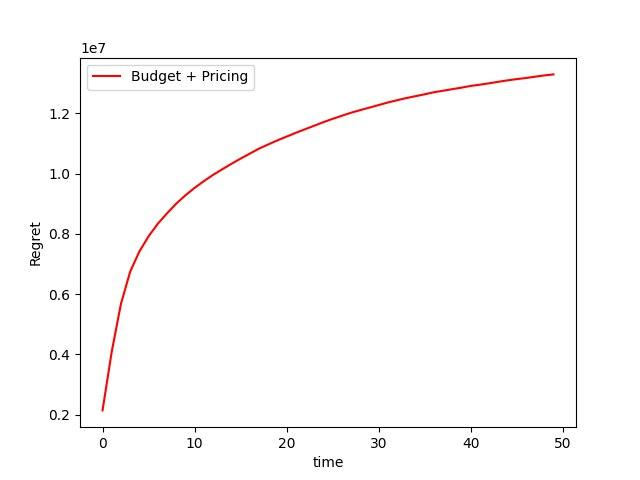
\includegraphics[width=0.80\textwidth]{sections/images/opt_constrained_regret.jpg}}
\end{figure}

\begin{figure}
    \caption{Reward}
    \label{fig:opt_constrained_reward}
    \makebox[\textwidth][c]{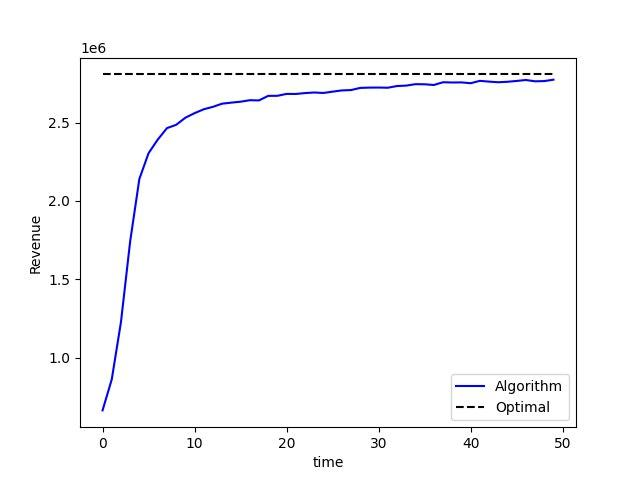
\includegraphics[width=0.80\textwidth]{sections/images/opt_constrained_reward.jpg}}
\end{figure}
\end{document}